%% ----------------------------------------------------------------
%% Thesis.tex -- main
%% ---------------------------------------------------------------- 

\documentclass[a4paper, 10pt, oneside]{memoir}
%% Use the option citeauthor to be able to use citet. The default cite will still work.
\usepackage[citeauthor]{basilea}

%% ----------------------------------------------------------------

\title				{Freshness-aware Data Management in a Polystore system}
\thesistype			{Master thesis}

\department 		    {Department of Mathematics and Computer Science}
\faculty			{Faculty of Science of the University of Basel}
\research		    {Database and Information Systems Group\\dbis.dmi.unibas.ch}

\examiner    		{Prof. Dr. Heiko Schuldt}
\supervisor  		{Marco Vogt, MSc.}

\authors     		{Marc Hennemann}
\email				{marc.hennemann@stud.unibas.ch}
\immatriculnr		{19-067-586}

\date				{May 7, 2022}

% switch here for the german logo to logo-de
\ulogo				{Template/logo-en} 


%% ----------------------------------------------------------------
\begin{document}

% for english use \selectlanguage{english}, for german use \selectlanguage{ngerman}
\selectlanguage{english}

\thesisfront
\maketitle
\pagestyle{thesis}
%% ----------------------------------------------------------------
% !TEX root = ../Thesis.tex
\chapter{Acknowledgments}
So Long, and Thanks for All the Fish. And the template.
%% ----------------------------------------------------------------
% !TEX root = ../Thesis.tex
\chapter{Abstract}
This thesis discusses the thesis template using some examples of the Turing Machine.
%% ----------------------------------------------------------------
\thesistoc
%% ----------------------------------------------------------------
%\thesisnomencl
%% ----------------------------------------------------------------
\thesismain
% !TEX root = ../Thesis.tex
\chapter{Introduction}

This is the introduction to the thesis template. The goal is to give students a starting point on how to format and style their Bachelor or Master thesis\footnote{This document also shows how to use the template.}. 

Please make sure to always use the most current version of this template, by downloading it always from the original git repository:
\begin{center}
	\url{http://www.github.com/ivangiangreco/unibas-latex} 
\end{center}

We will use throughout this tutorial some references to Turing's imitation game~\cite{turing:1950} and the Turing machine~\cite{turing:1936}. You may be interested in reading these papers.

\vspace{1em}
The package comes with an option regarding the bibliography style.
You can include the package with
\begin{verbatim}
\usepackage[citeauthor]{basilea}
\end{verbatim}
to be able to cite authors directly with
\begin{verbatim}
\citet{turing:1950}
\end{verbatim}

If the option is enabled, then the following reference should print Turing [2]:~\citet{turing:1950}


% !TEX root = ../Thesis.tex
\chapter{Body of the Thesis}

This is the body of the thesis.

\section{Structure}
\label{sec:my-label}

\subsection{Sub-Section}

\subsubsection{Sub-Sub-Section}

\paragraph{Paragraph}

\subparagraph{Even Sub-Paragraph}

This is the body text. Make sure that when you reference anything you use labels and references. When you refer to anything, you normally capitalise the type of object you reference to, e.g. Section~\ref{sec:my-label} instead of section~\ref{sec:my-label}. You may also just use the \texttt{cref} command and it will generate the label, e.g., for \cref{sec:my-label}, we did not specify the word ``Section''.

Hint: Try to structure your labels as it is done with \texttt{sec:my-label} and \texttt{fig:machine}, etc.



\section{Equations}
A Turing Machine is a 7-Tuple:
\begin{equation}
    M = \langle Q, \Gamma, b, \Sigma, \delta, q_0, F \rangle
\end{equation}
A Turing Machine is a 7-Tuple even if defined in the text, as in $M = \langle Q, \Gamma, b, \Sigma, \delta, q_0, F \rangle$.




\section{Tables}
Some tables can also be used as shown in \cref{tab:table}\footnote{Table captions are normally above the table.}. Remember that tables might be positioned elsewhere in the document. You can force positioning by putting a \texttt{ht!} in the definition.

\begin{table}[ht!]
\centering
\caption{Frequency of Paper Citations. By the way: Make sure to put the label always after the caption, otherwise \LaTeX{} might reference wrongly!}
\begin{tabular}{lcl} \toprule
Title&$f$&Comments\\ \midrule
The chemical basis of morphogenesis & 7327 & \\ 
On computable numbers, with an application to the ... & 6347 & Turing Machine\\
Computing machinery and intelligence & 6130 & \\ \bottomrule
\end{tabular}
\label{tab:table}
\end{table}




\section{Figures}
Figures are nice to show concepts visually. For organising well your thesis, put all figures in the Figures folder. Figure~\ref{fig:machine} shows how to insert an image into your document. \Cref{fig:tm} references a figure with multiple sub-figures, whereas the sub-figures are referenced by \cref{fig:tm:tm1}, etc. \todoMissing{Description of figure.}

\begin{figure}
\centering
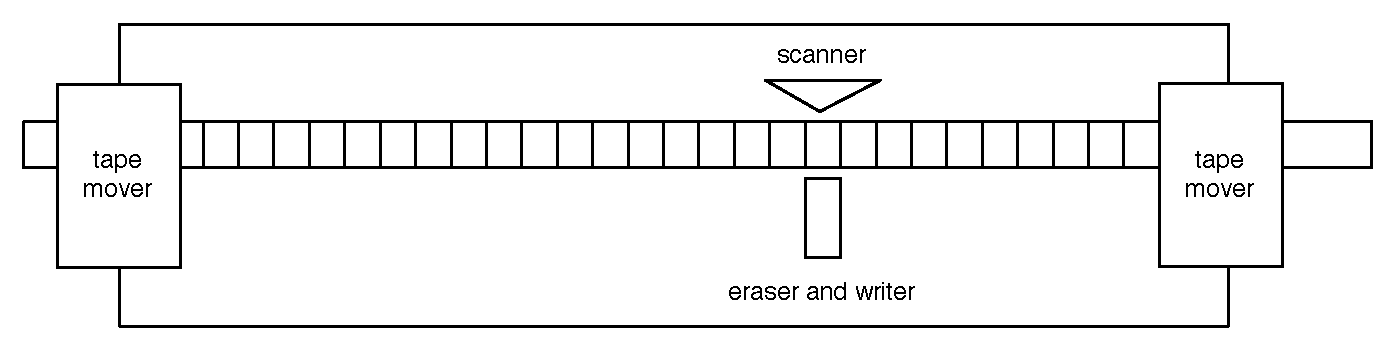
\includegraphics[width=0.9\textwidth]{turingmachine}
\caption{A Turing machine.}
\label{fig:machine}
\end{figure}


\begin{figure}
\centering
\subbottom[Turing Machine 1\label{fig:tm:tm1}]{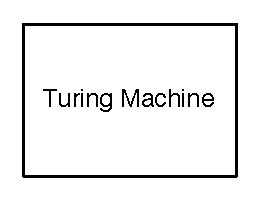
\includegraphics[width=0.2\textwidth]{block}}
\subbottom[Turing Machine 2\label{fig:tm:tm2}]{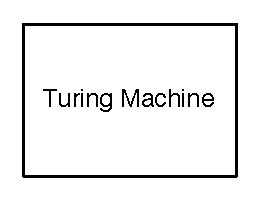
\includegraphics[width=0.2\textwidth]{block}}
\subbottom[Turing Machine 3\label{fig:tm:tm3}]{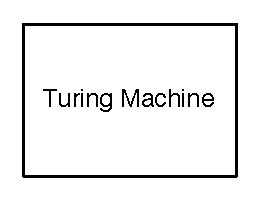
\includegraphics[width=0.2\textwidth]{block}}
\subbottom[Turing Machine 4\label{fig:tm:tm4}]{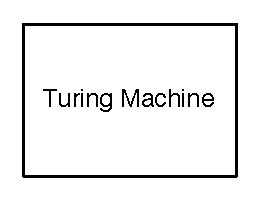
\includegraphics[width=0.2\textwidth]{block}}
\caption{Plots of four Turing machines}
\label{fig:tm}
\end{figure}




\section{Packages}
These packages might be helpful for writing your thesis:

\begin{description}
	\item[\texttt{caption}] to adjust the look of your captions
	\item[\texttt{glossaries}] for creating glossaries (also list of symbols)
	\item[\texttt{makeidx}] for indexes and the back of your document
	\item[\texttt{algorithm, algorithmicx, algpseudocode}] for adding algorithms to your document
\end{description}
% !TEX root = ../Thesis.tex
\chapter{Conclusion}
This is a short conclusion on the thesis template documentation. If you have any comments or suggestions for improving the template, if you find any bugs or problems, please contact me. 

\vspace{2cm}

Good luck with your thesis!
% !TEX root = ../Thesis.tex
\chapter{Introduction}
\label{c:intro}

Over the last decade, cloud computing has become a crucial and central part in the industry \cite{claremont:2005}.
This technological advancement in infrastructure layouts allows companies to rent software as well as hardware resources to
build and compose their entire data center virtually in the cloud,
without having to invest in expensive hardware and location to maintain their compute resources
solely on premise. These providers usually maintain different distributed data centers 
across the globe and provide private or shared access on their available resources according
to their Service Level Agreement (SLA). Such guarantees in quality-of-service (QoS) usually 
include elastic up- and down-scaling of rented resources and a high degree of availability 
which is achieved by replicating data across different regions \cite{terry:2013}. 

Ever since the rise of the \emph{Big Data} era, these providers are faced with continuous
and rapidly growing heterogeneous datasets. These are accompanied by widely varying requirements 
and characteristics for data driven applications. This increased the need to leverage custom-tailored 
database systems to gain meaningful insights on their data as quickly as possible.

To efficiently process and extract relevant information out of these data silos new systems
have emerged, which exactly aim to provide a solution for these new 
demands on varying workloads and ever-growing data sources.

Such novel Polystore systems aim to combine several physical data engines to enable various
new possibilities, to provide the best response times for each use case by exploiting
the key benefits of each engine \cite{stonebraker:2005}. Although these data management systems are inherently
built to process heterogeneous data with high throughput, the amount of produced data
still continues to grow.
Therefore, the importance of accessing the right data efficiently is crucial
for organizations to stay economical and competitive. Cloud providers which offer such systems consequently 
need reliable functionality to manage these large volumes of data to not waste useful computations and time when users
try to retrieve relevant data \cite{levandowski2013}.
To comply with their QoS requirements and sufficiently provide acceptable access times for their services, 
they have come up with data freshness strategies as an important part of data management in a
distributed setup. 
The freshness in such a case reflects how current and up-to-date a data item is.
Since not all applications pursue the same goals, they often depend on different levels of freshness which can be used to identify a well-suited location
to retrieve the data. This ultimately mitigates the need to always update every existing data replica to the most recent state and defer changes until
it is processable by the underlying system.
Such delayed updates allow for much higher throughput and increased performance, in use cases were also slightly outdated data 
is acceptable.

\section{Goal?}

\section{Contribution}
This report contributes as a preparation for a masters thesis. To identify necessary requirements to implemented and design possible 
freshness variations in a polystore system. Several aspects of previous published research work is compared and considered when adapting it to polystore systems.

\section{Outline}
This report is structured as follows:
In chapter \ref{c:related} the foundations and concepts of data freshness characteristics are presented.
We give an overview over the current state of research in the field of data freshness.
Chapter \ref{c:propositions} describes the necessary requirements to introduce the notion of freshness inside a polystore system. Additionally, it proposes and discusses
possible approaches how to implement them in Polypheny-DB.
While chapter \ref{c:evaluation} focuses on possibilities how to ensure correctness and measure the performance of an implementation, including all necessary prerequisites.
Finally, chapter \ref{c:plan} concludes the report by defining individual workpackages according to the proposed
implementations and gives a coarse roadmap how the project will be structured and carried out.



% !TEX root = ../Thesis.tex

\chapter{Related work}
\label{c:related}

This chapter aims to provide a background for the given topics as well as talking about the related and recent research activities for the respective sections.


To ensure the overall consistency of a system, current approaches in cloud environments use well-established protocols with unified blocking behaviours. 
This includes Strict two phase locking (S2PL) for correct serializability treatment as well as two-phase commit (2PC) for global atomicity in a distributed database 
setup. Such mechanisms are mainly utilized when updates and changes to the system are replicated eagerly to every available replica to maintain a consistent state
while complying with the common ACID properties \cite{tamer:2005}.
However, these  directly impact and ultimately mitigate the availability and response time agreements of most service providers.
Hence, different approaches were created which aim to relax the strict ACID properties towards the rather loose BASE ones.
BASE in this context stands for \textbf{B}asically \textbf{A}vailable \textbf{S}oft State and \textbf{E}ventual Consistency\cite{shapiro:2011}.
To implement this concept, updates on data items do not need to be executed immediately on every participating node.
It is sufficient to apply the change only on a few nodes and deferring the data replication to a point in time when the workload on the system is low and 
resources are not occupied by client requests. This form of lazily replication can drastically increase the performance while also reducing the costs of maintaining
all replicas at once. However, since these client requests are not serialized anymore this could lead to users accessing outdated and stale data items
which have not been updated yet.
As a consequence of lazy replication the system now persists multiple versions of data objects which logically reflect the data freshness.
Voicu et al. \cite{voicu:2010} suggest that since not all applications need the most up-to-date data, one could easily exploit 
this side effect by keeping several replicas of a datum as different levels of freshness.
This notion of or recency can then be utilized to ease the selection of correct replicas to fulfil individual client requests which even tolerate stale data as well.
For cloud providers this combination of eager and lazy replication together with the resulting different stages of freshness 
offers a great trade off between latency and access time for freshness and enables efficient usage of available resources.


\section{Data Freshness}
The idea of freshness is a widely used concept among distributed data integration systems and intuitively introduces the idea of how old or stale data is.
However, several notions and interpretations how to characterize and measure data freshness exist.
In 1999 Naumann et al. \cite{naumann:1999} already stated that although the idea of data quality and freshness has no commonly agreed definition and varies
among use cases it is strongly related to the concept of accuracy. Such accuracy of a data object can roughly be summarized as the percentage of 
objects without data change. This thought was also shared by the author of \cite{redman:1996}  who defined the data accuracy as "the degree of agreement between 
collection of data values and a source agreed to be correct".
Hence it can therefore be considered as the precision and accuracy of such data elements in respect to its most up-to-date version.
This approach is now commonly used among distributed systems which compare replicas with a designated "single source of truth" or some defined 
primary or leader nodes in such a setup. Referring to freshness as a measure of the divergence between a replica and the current value. 

Such strong application driven requirements call for a dedicated data model which represents the handling of data in a system which has
freshness related requirements on arbitrary data items.


Peralta \cite{peralta:2006} also described freshness as a matter of how old data is and linked this to an users expectation who is interested in when the data was produced
or if there may be other sources that have more recent or different kinds of freshness. 
Consequently using the last time objects were updated, to identify any accuracy measures. Peralta also distinguished between two quality factors. 
The \emph{Currency factor} which expresses how stale data is after it has been extracted and
delivered to the user. This concept is often considered in Data Warehousing systems, when already extracted materialized data is processed and delivered to the user 
while the source data might have already been updated after it has initially been extracted and materialized resulting in stale data.
The second factor corresponds to the \emph{timeliness} of data. It essentially states how old data is and captures the gap between the last update and delivery.


\section{Freshness analysis and metrics}
\label{r:freshness_metrics}
A metric is a specific figure which can be used to evaluate given quality factors.
With the various definitions and approaches to data freshness itself, the metrics to identify and measure the level of freshness also vary.
Several metrics are summarized by \cite{cho:2000}\cite{pacitti:2000}\cite{peralta:2006} and can be categorized as:
\begin{itemize}
    \item \textbf{Currency metric}: Measures the elapsed time since the source data changed without being reflected in a materialized view or a replica in distributed setups.
    \item \textbf{Obsolence metric}: Which accumulates the number of updates to a source since the data extraction time. For replicated systems this can be characterized as the 
    number of updates that still need to be applied to a secondary system after it has been refreshed.
    \item \textbf{Freshness-ratio metric}: Identifies the percentage of extracted elements that are indeed up-to-date compared to their current values.
    \item \textbf{Timeliness metric}: Measures the time that has elapsed since the data was updated. Generally defined as the time when the replica was last updated.
\end{itemize}



While \cite{bedewy:2016} and \cite{zhong:2018} define the notion of freshness by relating it to the age-of-information (AoI) respectiviely the timeliness represented by 
the timestamp of the transactions which has updated the value has as well as the age-of-synchronization (AoS) which corresponds to the time when the value was updated.



\subsection{How to express freshness}
\label{r:express_freshness}

Along the various freshness metrics as described in \ref{r:freshness_metrics}, Tamer et al. \cite{tamer:2005} list three types of freshness constraints that users could specify to
suggest an accepted level of freshness.
\begin{itemize}
    \item \textbf{Time-bound constraints}: Are used as timestamp that tolerate values which were updated by younger transactions. 

    \item \textbf{Value-bound constraints}: Consider percentage deviation from the current value. This is more commonly used with numbers than with text and is considered to
    be mutually consistent if the values do not diverge more than a certain amount.

    \item \textbf{Drift constraints on multiple data items}: Relevant for transactions which read multiple data items. It is acceptable for users if the update timestamps 
    of all data items are all within the same specified interval. Additionally for aggregations, as long as a particular aggregate computation 
    is within a tolerable range it can be accepted. Even if some individual values of the data items are more out of sync than the compound operation.

\end{itemize}

The notion of time-bound constraints is also shared by the authors of \cite{voicu:2010}. They propose to measure and specify these freshness constraints 
with the notion of \emph{absolute-} and \emph{delay freshness} to characterize their proposed freshness functionalities.

Here the \textbf{Absolute Freshness} of a data item \textbf{d} is characterized by its timestamp \textbf{t}
of the most recent committed update transaction that has updated the item \textbf{d}.
These timestamps can be used by the client to individually define their freshness requirements. The younger a timestamp the fresher the data.
Additionally they use \textbf{Delay Freshness} to define how old and outdated requested data objects $t(d)$ are compared to the commit time of the current value $t(d_0)$.
Defining their freshness function as $f(d) = \frac{t(d)}{t(d_0)}, with f(d) \in [0,1]$ resulting in a \emph{freshness index}.
Röhm et al. \cite{rohm:2002} state that such an index consequently reflects how much the data has deviated from its up-to-date version.
An index of 1 intuitively means that the data is at its most recent state, while an index of 0 is defined as infinitely outdated.

While \cite{xiang:2008} and \cite{fekete:2018} both consider the delay-based staleness in the time domain as well they also consider constraints on 
an acceptable value-based divergence $\delta$. This aims to to measure the difference between two numerical values by anlyzing their similarity on basis of their 
absolute value $|d_0 - d| < \delta $. Low values between base and replicated data reflects a more up-to-date replica for a given object.




\section{Update propagation - Replication}
\label{r:replication}
An essential part to gain performance with freshness-aware data management is loosening the update situations by reducing the number of 
replicas which need to be updated. This decoupling between necessary updates on a primary site and deferred updates towards secondaries 
reduces the total update time and in contrast increases the overall availability of the database system.
This mechanism itself suggests to the user that the database system is updated eagerly while internally the updates are actually propagated lazily. 
Although this has the side effect that secondaries exist which hold slightly outdated and stale data. 
Due to the decoupling these can now efficiently be utilized as read-only copies to speed up OLAP workload while still performing transactional processing 
at primary level as \cite{psaroudakis:2015} \cite{rohm:2002} \cite{xiang:2008} have pointed out in their work.

Depending on the architectural setup different refreshment strategies have been proposed how updates are propagated towards outdated nodes.

Wei et al. \cite{wei:2004} propose a replication in form of an update policy adaptation algorithm that dynamically selects update policies
for derived data items according to system conditions to have several layers of validation transaction to be fulfilled to actually be executed.
E.g. in the validation stage, the system checks the freshness of the accessed data. If this accessed data is not fresh enough the entire transactions will be restarted.
This imposes a huge performance mitigation since the transaction itself could be handled multiple times before it might actually get executed.

Psaroudakis et al. \cite{psaroudakis:2015} mention the existing design gaps between OLTP- and OLAP-oriented DBMS and describe the importance of allowing the execution of
OLAP queries even during the execution of transactional workload. However, their focus here rather resides on a single table level than on a replication scenario in a distributed 
environement. Furthermore, they are interested in real-time processing and claim that even the slightest outdated data is unacceptable to provide real-time reporting.
To fulfil these mixed workload requirements they described the idea of SAP HANA to offer a main area which contains the base data and a delta area 
which supports transactional operations and includes recently changed data. Read operations need to query main and delta jointly to provide results. 
Since the delta area could increase without bound it is periodically merged into the main section. 


A similar approach is shared in \cite{wei:2004} which aimed to mitigate complexity and replication overhead by combining base data elements and derived elements.
For queries a base set of information is enriched with a delta to get the relevant derived output.
This reduces the needed update cycles on all replicas since base information is always available and queued changes are applied during runtime to recompute 
the actual response. However, this approach is costly when encompassing several derived data sets and is therefore rather suited for values that can 
easily be derived. 


To increase the transactional throughput \cite{pacitti:2005} Pacitti et al. introduce concurrent replica refreshments and discuss the idea of \emph{Preventive Replication} 
by using an asynchronous primary-copy replication approach and still being able to enforce strong consistency. This is achieved by utilizing a First-In First-Out Queue (FIFO) queue 
to correctly serialize any updates which shall be delivered to secondary replicas.

The authors in \cite{voicu:2010} propose several multi-tier layers to handle replication and freshness scores. Nodes are classified into two categories either as updatable or read-only
and placed onto three levels.
Level-1 nodes receive updates acting as primary servers, level-2 sites are read-only nodes containing as up-to-date data as possible and level-3 read-only nodes
where data is not updated frequently. These levels are layered and composed as a tree receiving asynchronous updates from the lower level. 
The higher the level, the more outdated the data.

In contrast, \cite{xiang:2008} approaches its replication algorithm with a relationship between data items by utilizing a directed acyclic graph (DAG).
Their graph essentially denotes a dependency between data items. The root node of such graphs corresponds to a base data item and child nodes correspond 
to its deviations over time. This as well corresponds to a multilayer replication setup.






\subsection{Refresh strategies}
\label{r:strategies}
Based on the discussed lazy propagation mechanisms in \ref{r:replication}, three refresh and update strategies could be identified when updates should be propagated 
to replicas.

Although the authors of \cite{psaroudakis:2015} rather focus on table-level objects and not on replication scenarios the up-date mechanism 
still follows the same requirements to jointly support a mixed workload of OLTP- and OLAP-oriented transactions.
It considers a periodic approach when the main and delta areas shall be merged which essentially refers to updating an outdated base item, respectively the main area.

Others \cite{rohm:2002} avoid the scheduling of such update propagations completely by simply decoupling the primary update transactions from the read-only nodes
and immediately executing the propagation-transactions as well. Although this helps the throughput of the initial update transactions the secondaries do not really 
stay outdated for any time at all. Since, such approaches as well as periodic scheduling completely neglect to verify the load on the underlying system it could 
cause unnecessary resource consumption on the replicas to be updated. Therefore, this should always be accompanied by identifying the idle time of replicas as well 
as ensuring that the current load on the replicas not to high and is therefore able to endure such an update \cite{voicu:2010}.

Contrary to \cite{peralta:2006} which talks about determining the goal to identify the minimum set of refresh transactions such that it is guaranteed that a node contains 
sufficiently fresh data with respect of the users requirements. Any outdated node independently will pull the number of updates which is required to fulfil future requests 
of such requirements.

Wei et al. \cite{wei:2004} follow a slightly different approach by analyzing the \emph{Access Update Ratio} (AUR) for any data object \textbf{d} which is given as: 
$AUR(d) = \frac{AccessFrequency(d)}{UpdateFrequency(d)}$. Consequently any item above an AUR of 1 is considered to be accessed at least as frequently as it is updated
and is considered as hot and shall be updated as soon as possible for applications to receive the real-time value. 
Whereas a ratio below this threshold refers to cold data and takes into account that this is accessed rather infrequently and thus needs no immediate refresh. 







\section{Consistency}
There are several constraints to consider that need to ensure the consistency in a distributed setup. In general two requirements can be defined that have to be fulfilled to
guarantee correctness in respect of freshness. For one, transactions that refresh stores need to be executed on all read-only nodes in the same serialization order as the 
original update transaction. Secondly all queries of a read transaction must access data with the same freshness.


The authors of \cite{xiang:2008}\cite{wei:2004} considered data freshness together with the scheduling of update transactions and talked about its freshness from the 
point of view of real time applications. They considered the concept of temporal validity in context of value-based freshness,
such that specific values are only valid for a certain time interval before they become outdated. Hence, it is necessary to classify objects into
temporal data that can continuously change to reflect a real world state and non-temporal objects than will not become outdated overtime like the validity of an ID card.
This concept essentially pursues the fundamentals of temporal databases, which keep historic values as well as their validity-intervals, to allow reconstruction of any 
past value \cite{etzion:1998}. 

Voicu et al. \cite{voicu:2010} propose a decoupling of transactions to correctly separate the individual requirements for update propagations.
These transactions are differentiated in regular update transactions that target primary nodes, propagation transactions that refresh read-only nodes, 
refresh transactions that are executed if a freshness level on a local store cannot be provided and finally OLAP related read-only transactions.
Furthermore, they require that data accessed within a transaction is consistent, independent of its freshness. To correctly serialize the updates
they ensure that their update serialization order is the commit order of the initial update transactions.

The authors of \cite{psaroudakis:2015} introduced a common data structure for both workloads for delta and
main store and the usage of Muti Version Concurrency Control (MVCC) to provide access for both OLTP and OLAP.
This implicitly enables the system to keep several versions of a data item.
These versions can be directly used as outdated or freshness guarantees. However, the implementation of MVCC is complex and needs more system resources.
Although this would indeed improve update times and would support referential integrity. 

Finally, the authors of \cite{akal:2005} propose freshness locks which are applied to the stores which have been selected to fulfil the read requests. 
These locks aim to provide fast response times for OLAP workload and ensure that data is not refreshed when beeing read within one transaction.



\section{Freshness-aware Read Access}
\label{r:read}
Since the essential idea of data freshness revolves around fast read access while transactional workload is currently beeing executed,
the read access is a matter of efficiently routing any client request to a suitable replica in respect of the required level of freshness.
According to \cite{rohm:2002} a router needs to utilize system state information on replicas to identify the correct way to route a query.

In \cite{voicu:2010} clients can directly contact any read-only replica. For every read-only transaction they can as well specify
their tolerated freshness level, by specifying a timestamp which is internally converted to a freshness index. If the replica is able to fulfil the request 
it directly returns the response to the client. If it currently does not posses a sufficent freshness level it routes the request to another node which can be identified 
by routing it towards the root of the tree. The parent is able to identify which node is able to fulfil the condition.  
If none of the nodes are able to fulfil the request in this subtree a refresh transaction is executed updating all nodes before processing the read operation.

The authors \cite{huang:2020} introduce a central \emph{preference manager as a service} at the client site. This manager is able to suggest where to route queries 
based on given cost metrics and by comparing latencies for any request to improve the overall performance to deliberately choose if a request shall be routed to a 
primary or secondary site. This analysis is influenced by the \emph{Replication Lag} inside a MongoDB cluster and refers to the average time how much time passes 
before an update is propagated to the secondaries. 





% !TEX root = ../Thesis.tex
\chapter{System Architecture}
\label{c:architecture}

In this chapter we briefly describe and illustrate a simplified version of Polyphenys current architecture.\\

\todoMissing{Polypheny multi-model teherfore tables are considered entities }

\section{Polypheny-DB}
PolyDBMS \cite{polypheny2021}
\todo{Add PolyDBMS cite Love Marriage or Marriage of convenience}

\textit{Polypheny-DB} is an Open-Source project\footnote{https://polypheny.org/} developed by 
the \textit{Database and Information Systems} (DBIS) group of the University of Basel.\\

Polypheny-DB is a self-adaptive polystore that provides cost- and workload aware access to heterogeneous data\cite{poly2020}.

Compared to other systems like \textit{C-Store}\cite{cstore_2005} or \textit{SAP HANA} \cite{hana_2012}, 
Polypheny-DB does not provide its own set of different storage engines to support 
different workload demands.\\
Instead, it acts as a higher-order DBMS which provides a single-entry point to 
a variety of possible databases like 
\textit{Cassandra}\footnote{https://cassandra.apache.org/}, 
\textit{PostgreSQL}\footnote{https://www.postgresql.org/} 
and \textit{MonetDB}\footnote{https://www.monetdb.org/}. 
These can be integrated, attached and managed by Polypheny-DB which will incorporate the underlying 
heterogenous data storage engines with their different data structures. It is 
desigend to abstract applications from the physical execution engine while profiting from 
performance improvements through cross-engine executions. 
\\
For incoming queries Polypheny-DB's routing engine will automatically analyze the query and decide 
which store will provide the best response. The query is then explicitly routed to these data stores. 
This approach can be characterized as a dynamically optimizing data management layer for different workloads.

\subsection{Data Placements}
\subsubsection{Vertical Placements}
\subsubsection{Data Placements}

\subsection{Query Routing}



% !TEX root = ../Thesis.tex
\chapter{Propositions}
\label{c:propositions}

This chapter is separated into several sections were each represents a necessary building block to provide the notion of data fresh in Polypheny-DB.
These blocks are compared and discussed to the implementations presented in \ref{c:related} to propose approaches how such techniques could be applied to polystore
systems. Essentially we have to think about how we want to express freshness, find a suitable metric to measure it and provide users a possibility to formulate 
an acceptable level of freshness. Based on these fundamentals we need to consider how update transactions can be decoupled and deferred, how replicas will
be refreshed while ensuring the consistency of the system and how to enable the routing to identify freshness levels to speed up read-only operations. 



\section{ How to express freshness}
\label{express}

As discussed in \ref{r:express_freshness}, freshness can be expressed via several indications.
Although we have described a number of domains only the time-bound constraints will be pursuit further. 
While freshness extractions on value-based divergence is only really suitable for numerical values
to calculate the percentage of deviations from the base item, time-based freshness can be applied to arbitrary types and can therefore be used 
in a more general notion. 
Such time-bound constraints allow to utilize timestamps as well as the usage of freshness indexes when referring to a desired level of freshness. 
Although a timestamp can be used more intuitively, an index is abstract and can therefore be generally applied without having to specify an absolute time dependency.

Hence, we propose that users can specify their tolerated level of freshness in a variety of ways. For one we want to provide the possibility to let users 
request their accepted level of freshness as an attachment to the query language. This can be achieved by extending the query functionality of Polypheny-DB.
Such constraints can either be formulated by providing a timestamp to implicitly give an accepted lower bound on an absolute time.
Additionally, time delays such as \textit{"Last 30 minutes"} can be specified to request a relative freshness level.
Finally, by directly requesting a desired level of freshness defined as a percentage value, meaning a value of 70\% would tolerate data objects
with a flexible accuracy of 30\% outdated data corresponding to the time since the primary copy has been updated.
However, internally all specifications are converted into freshness indexes since they are independent of any time window and can be constructed, compared and applied 
without any restrictive dependencies.\\

Moreover, to improve the user experience we consider to enrich the query tree paths to specify which level of freshness was requested and with which level it was 
ultimately fulfilled. Furthermore, for successfully executed queries that considered some kind of freshness it shall be added in the SQL response that is has been 
executed by means of a specific freshness level.
In such a way a user can not only steer its desire but is also informed whether the request could be fulfilled.




\section{ Replication Roles }
\label{roles}

As already discussed in the implementations in \ref{r:strategies} it is crucial to define and assign roles to loosen the locking situation on nodes
to minimize update times over all. The related work clearly separated between primary-update nodes and read-only nodes, where 
read-only nodes cannot be directly updated by the user and will only receive refresh updates internally by the primary nodes.
Therefore, these are the only nodes used for read-operations. 
However, we want to include primary nodes for reads as well and therefore propose the naming-convention in respect of the desired state as \emph{up-to-date nodes} for primaries
and \emph{outdated-nodes} referring to any secondary node. \\
With the introduced changes to internal partitioning described in \cite{hennemann_2021}, we now have the possibility to utilize the notion of \emph{Partition Groups}
to label stores with desired state respectively their roles.  
When deciding to use freshness on an object, administrators should be able to define how many replication tiers they want to have in a particular setup.
The minimum requirement is always a complete primary up-to-date node, either as a full placement or composed out of several vertical partitions and one outdated node.  
However, to support a multi-tier approach as \cite{voicu:2010}, outdated nodes can occur multiple times and can hold different levels of freshness with any number of vertically partitioned
placements. Therefore, a suitable mechanism has to be introduced which enables the definition of replication orders and paths. This could then be used to 
intuitively have placements at different freshness levels resulting in tertiary adapters only being updated by secondaries.\\







\section{Replication}
\label{replication}
Since data freshness occurs as a side effect of using lazy replication and can therefore already
be used as a consequence of saving workload when not needing to update every replica eagerly.
As suggested in \ref{r:replication} there exist several techniques how outdated nodes can be updated lazyily in the context of freshness.
Most of these presented distributed architectures follow a primary-copy approach for master-driven replication to all their secondary replicas.
This eases the the control and flow of data. Although in the proposed works some systems allowed to access read-only copies directly
with Polypheny-DB we always have a single point of entry which can vaguely be compared as the poly-layer acting as a master node
when distributing or even routing queries. Hence Polypheny acts as the master anyway. However since any requests have to pass through the poly-layer
we have full control how and where queries need to be routed to allowing us to selectively route read-operations to outdated and up-to-date stores alike.
This enables Polypheny-DB to take full control how different levels of data freshness are being accessed.

With this abstraction layer on top of the stores we can leverage the DBMS to act as a coordination service allowing us to loosen the eager replications and 
locking mechanisms to be restricted to the primary nodes only. Currently, one has to wait until an update is persisted everywhere and are therefore
dependened on slowest performing store.
To mitigate this behaviour we want to decouple the commonly used update transactions and logically divide it into a total of three separate transactions types
to allow deferred refreshments of objects.
\begin{itemize}
    \item \textbf{Update transaction}: Consequently are write operations that are targeted on primary placements only.
    \item \textbf{Propagation transaction}: Belong to a refresh operation updating the data freshness of an outdated secondary node which is 
    executed automatically by the system.
    \item \textbf{Refresh transaction}: A propagation transaction which is manually triggered by a user to refresh the data on an arbitrary outdated node.
\end{itemize}

Allthough, logically being used differently they are technically executed with the same capabilities and only really separate in terms of locking.
They are rather used as a clear indication on which part of the process is referred.

These changes will also have an impact on the partition distribution constraints. For vertically and horizontally partitioned 
entities this means that all constraints on the number of available column-placements can only be considered for primary update stores. Otherwise, this could harm
the consistency of the system. For nodes labeled as outdated any variation is possible.

\subsection{Update Propagation}
We have several possibilities how to handle and propagate the updates.
Since every write-operation needs to go through Polypheny, we can easily keep track which operations have been applied to the primary server and when 
they need to be applied to the secondaries. Essentially every possible solution needs some form of queue to store updates that still need to be executed 
on secondaries. For correct serializability it is sufficient to store the commit timestamp of the update transaction with each queue item. This imposes a natural
execution order of any item in the queue to be delivered to the secondaries.
We propose the following approaches: \\

\textbf{CDC (Change Data Capture)}\\
We can implement the notion of a shadow table which is filled by trigger on the base table.
As soon as the base table gets modified by an update transaction any changes applied are stored and consequently tracked.
Accompanied by a commit-timestamp its content is then used inside propagation transactions to refresh outdated placements.
Once placements are updated the propagated entries inside the shadow table are deleted. 
This has the advantage that we can utilize a common datastructure in Polypheny out-of-the-box without having to implement any further activities.
It is persisted and available after a downtime which ensures the recoverability of the system.
However since this results is generating several statements that essentially has to traverse the entire system in order to be executed this could lead to 
large overhead in the system which could impact the performance as well as requiring more resources.
Furthermore, since this is an updatable table the implemented locking mechanisms has to be applied as well. This excessive accessing however could result in high 
locking situations and therefore again impact the update time after all.\\

\textbf{Internal structure}\\
Another possibility would be to handle this approach entirely with internal structures.
For example with the implementation of a MOM (Message Oriented Middleware) between the poly-layer and available adapters. The initial update transactions can append 
the changes into a persistent queue. This queue can then be asynchronously queried using a pull-based approach on adapter site to apply all changes necessary for them. \\

\textbf{Internal Partitions} \\
Another propositions would be the usage of background processing together with physical partitions. Although, they were originally intended to serve the horizontal partition 
use case they are internally configured to represent a physical table. Partitions could be extended to be used as general system internals
which are accompanied by an update-timestamp that represents the last time the partition has been updated, this could include the Age-of-Information as well as 
the Age-of-Synchronization. Furthermore, since partitions logically belong to partition groups described in \ref{express} we can easily identify which partitions are considered to be 
outdated or should always be up-to-date. With these information we could even use the existing capabilities of the \emph{Partition Manager} which uses the notion of 
partition-qualifiers to identify required levels of freshness.

For every update-transaction the eager replication is loosend to only consider the primary partitions for updates.
For the refresh operation itself we can utilize the \emph{Data Migrator} to extract the relevant data via an accumulated select-statement on the primary placements.
Additionally, to further decouple the data refreshment a hidden shadow partition can be created for this purpose. In that way writes on the primary copy as well as the 
currently existing outdated placements can still be executed while the outdated placement gets refreshed in the background. Once the data migration process has finished, 
we only need to logically apply a \emph{Refresh-Lock} to ensure the overall consistency. During the short time the outdated-site is locked the old placement is dropped and 
the hidden shadow partition is officially being activated. Since this only really requires one select on the primary site, write-operations can still take place, reducing
locks to a minimum. Even during the time the refresh-lock is active the benefits of the poly-layer comes in to play which enables the system to choose to 
route read-operations to primary servers as well.\\


\textbf{View Materialization}:\\
Along the idea of internal partitions materialization could help reduce the number of statements necessary to create new levels of freshness.
Since materialized views are considered to be snapshots of data objects, anytime a propagation or refresh operation is being executed a new materialized view is 
generated on basis of the up-to-date placement.
This would ommit replication operations entirely hence no bookkeeping of the queued updates would be necessary. The only needed reference would be the new timestamp
to calculate the freshness index.

As with the handling of internal partitions this can also be done entirely in the background. This limits the locking time to a minimum and is therefore only really 
necessary when switching the outdated with a refreshed view.
Allthough, one of the biggest downsides of materialization is the large additional resource consumption on storage, it can be neglected for polystore systems, since they are
inherently distributed and would otherwise store the entire content of the table. Therefore, it would even slightly reduce the data footprint on outdated placements.







\subsection{Refresh strategies}
As already stated above, there are essentially three ways to update a secondary node. 
For the automatic execution of propagation transactions a periodic execution has several downsides hence we propose to schedule
refreshment on the basis of the load on the outdated placements. Therefore, we will extend the adapter of the underlying stores to gather metrics on current workload
average response times in order to enable the poly-layer to decide based on this metrics when it is suitable to carry out a propagation-transaction.


Since it might be possible that a user may consider refreshing a placement manually, we have proposed refresh transactions. With this a user has the possibility to refresh
any replicas which are classified as outdated to a specific freshness level.
\begin{verbatim}
ALTER TABLE dummy REFRESH PLACEMENT ON STORE outdated_store 
UNTIL <TIMESTAMP>;
\end{verbatim}
Without any specification the placements shall be updated to the most recent state of the up-to-date version:
\begin{verbatim}
ALTER TABLE dummy REFRESH PLACEMENT ON STORE outdated_store;
\end{verbatim}

For this operation only freshness levels greater than the current local freshness level can be considered.
Furthermore, this should also provide the possibility to refresh all placements of an object.
\begin{verbatim}
ALTER TABLE dummy REFRESH ALL PLACEMENTS;
\end{verbatim}

Although such refresh-transactions can be executed on any placement, it will have no effect on primaries and simply omit their execution. 




\subsection{ Identify stale data }
\label{stale}

A prerequisite for the automatic execution of propagtion transactions is the identification of stale and outdated placements.
Although a trivial option would be to use the roles described in \ref{roles} and periodically gather all labeled placements, this would not scale much
considering a large amount of tables with at least one additional replica per table.\\

One proposition would be after every update transaction has commited to immediately inform dedicated notification services which will instantly trigger 
a load analysis on stores to be replicated. A sligthly different approach would be a central gossiping service as an adapter extension that gathers store metrics 
and declares them as idle, or loaded. With such a mechanism the notification service which received the information to update stores would not start querying a server
again and can directly utilize the pre-gathered metrics and choose to execute the update or defer it again.\\

Another approach to identify and update stale placements would be the idea to use update-on-read. Everytime a node flaged as outdated is used to serve a 
read-operation the level of freshness can be checked. If identified as outdated this could then trigger any of the propagation transactions proposed in 
\ref{r:strategies}. This would completely omit periodic background scheduling and would shorten processing time.\\
 
However, for both cases in terms of the resulting refresh rate we still have to consider if the change data becomes too large the refreshes tend to take longer.
So countermeasures have to be defined to minimize errors or downtimes.






\section{ Transactional guarantees }
\label{consistency}

To support the overall consistency of the system we have to ensure that all updates are correctly serialized and applied to the system.

Polypheny for one ensures global atomicty by using the two-phase commit (2PC) protocol and for correct isolation treatment
strong strict to phase locking (SS2PL). Currently, all placements are eagerly updated and locked whenever a write-operation is executed.
We need to loosen that constraints to increase update times and still ensure all transactional guarantees. The locking mechanism should therefore 
now only consider primary nodes. In that way we still can utilize secondaries with slightly outdated data for reads.\\

To ensure that the overall correctness of the system is maintained we will restrict the solution to allow freshness related parameters solely
for read-only transactions. For every update-transaction which considers freshness of any kind, consistency cannot be guaranteed since we might read outdated data
and use this data to write into another table. Therefore, we propose to enrich  the transactional context of Polypheny with a flag that states if any read-operation 
considers freshness. If this is the case, the update-transactions needs to be aborted.\\


Another important point to note is the referential integrity of outdated tables. We already ensured that outdated data cannot be used within update-transactions to 
ensure consistency and therefore guarantee correctness. However, for read-only transactions it should still be possible to join any tables while considering 
a desired level of freshness. 
Since it is rather complex and would result in refactoring the core of Polypheny-DBs, we currently refrain from supporting MVCC.
Hence, it might occur that cumulative reads on multiple objects might return incomplete results, since a specified freshness
level can be entirely different on two tables which makes it hard to even compare freshness levels among different objects. However since a user is willing to access 
stale data anyway this is a known risk and thus can be accepted.\\

Finally, as introduced in \ref{replication} the \emph{Refresh-Lock} is a newly introduced lock which holds the same characteristics as a regular lock on an object.
However, it shall only be applied whenever a refresh operation is currently in place. This way the routing mechanism can avoid sending any queries to that placement
for reads or a new refresh operation, which might have been triggered manually by an user.

To ensure the correct execution of refresh operations every placement that is outdated will receive an independent propagation- or refresh-transaction.
The serialization order of the updates to be executed is the commit order of the initial write transaction.
These can also be refreshed and updated independently which not only again reduces the total update time but also eases rollback scenarios.
Otherwise, we might need to define complex countermeasures to undo certain refreshes if one store was already refreshed but another has failed.




\section{ Freshness-aware Read Access }

With the description of \ref{express} how to explicitly express freshness, users have the ability to hint or even guide the routing process to select placements 
based on their desired freshness.\\
Users can choose to specify any tolerated level of freshness. The routing process analyzes this specification and gathers all placements which fulfil the necessary 
requirements by preferring secondary nodes labeled as outdated.
In case no secondary node can fulfil the request a primary placement is used to serve the query since they are not exclusive to receive updates such in other systems,
consequently utilizing all source available to the system.
Since only few systems presented in \ref{r:read} provided this functionality the routing process can be extended to support load balancing. 
With the proposed adapter background analysis the router can observe if any selected placement might be overloaded and therefore chooses to route 
queries to a different available location. \\



For the overall freshness guidance an extension of PolySQL is necessary.
Along the description in \ref{express} users can choose to select any of the specifications to guide the system.
\begin{verbatim}
SELECT * FROM dummy 
[ WITH FRESHNESS [ <TIMESTAMP> | <DELAY> | <PERCENTAGE> ] ];
\end{verbatim}
As an extension we also propose to omit the specifications entirely and only state to the system that any freshness level is acceptable or the system central
configured default, to further speed up queries.



As mentioned in \ref{consistency} since update transactions don't allow any usage of freshness metrics to ensure consistency, solely read-only transactions are allowed.
Hence, for read-operations on outdated nodes and data, locks can be omitted entirely since you will read stale data anyway.
We therefore only have to validate that no refresh-lock is currently in place.







\section{ Policies }

According to the idea, to generally relax consistency or allow a fine grained way of letting data owners decide what kind of consistency shall be desired for their object. 
Since freshness can be considered a trade-off between availability and consistency it is only fair to let users decide which level of consistency to enforce and 
how the freshness should be handled. We therefore propose the notion of policies to guide the system.
Policies are essentially intentions and desired states how the system should behave in various situations. 
The system can apply them when manual or automatic system maintenance is performed.
They shall therefore be introduced for any kind of configurable behaviour to allow any custom tailored behaviour. \\

Policies can be inherented and applied to any kind of object. When applied to a schema all entities inherent that polcies.
However, a different kind of policy with the same type can be applied to an entity overriding the one inherented by the parent.
Policies are about background processing how metadata and constraints on different objects are enforced. 
They provide a lightweight version of UDFs (User-Defined-Functions) to build custom-tailored behaviours into the system.
Other than the central configuration which is used to define core system behaviours. 
Such policies can be defined as:\\


\textbf{Consistency Policies}\\
Provide a notion of tuneable consistency, where users should be able to decide which levels to fulfill.
In such a case an adminsitrator could choose to define how many primary replicas an object should always contain.
This would directly impact the constraints on the table restricting users to remove more placements than defined by that policy.\\


\textbf{Freshness Policies}\\
Can be utilized to define behaviour on freshness related actions. As \cite{fekete:2018} stated it is crucial to define how far a replica can diverge from the true
and up-to-date value before a refresh transaction has to be critically executed.
Additionally, we could use these types of policies to let object owners define how their data shall be identified and consequently updates are propagated.
In such a way the system would stay customizable and would allow any methods discussed in \ref{stale} to be used dependent on the use case.
Considering how refreshes are triggered one policy for example might has chosen to defer a propagation transaction entirely hence it won't try again and
essentially waits for another chance when a new update-transaction is being executed and will trigger the service again. Another policy could suit other use cases better 
and assist by constantly querying the storages perfromance metrics to decide if an update should be executed.\\

Due to the inherent heterogenous nature of the polystore systems itself, use cases may widely vary. Hence, in gerneal there is no need to impose a 
general notion of freshness that is valid for all applications. Some might consider using CDC, while other prefer a partition approach or materialized views.
However, with policies these can all be implemented.\\


\subsection{Policy usage}

Since applications that are being served by polystores are very different to each other, they might have different requirements. 
Therefore, different object types shall be supported.

A policy shall generally be created inside a database.
\begin{verbatim}
CREATE POLICY policy_name as <configuration>;
\end{verbatim}

These policies can then be added to any object.
\begin{verbatim}
ALTER TABLE dummy ADD POLICY policy_name;
\end{verbatim}

Users should always be able to list information on all applied policies on any object.
\begin{verbatim}
SHOW POLICIES ON (DATABASE | SCHEMA | TABLE ) object_name;
\end{verbatim}


Furthermore they should be able to view the content of any policy: 
\begin{verbatim}
DESCRIBE POLICIY policy_name ON (DATABASE | SCHEMA | TABLE ) object_name; 
\end{verbatim}

To complement the idea of policies we also need a central \emph{Policy Manager} which ensures that the specified intentions are ensured.
The manager shall be added as an additional central component and acts as a verification layer whenever meta information on objects will change.


% !TEX root = ../Thesis.tex
\chapter{Evaluation}
\label{c:evaluation}

This chapter is separated into 

\section{Goal}
The evaluation has two goals the correctness as well as the impact of data freshness onto different kinds of workloads.

Verify and validate the correctness as well as the completeness of the implementation based on several characteristics.
These include the correct execution of lazy replication, the possibility to refresh statements on demand.

Impact of the replication engine on the underlying performance, if freshness indeed increases the overall parallel writes on the system.
Or if it is just marginally lower than before. Also compare this to the overall introduced overhead. And if the change was wort it

\section{Correctness}

\section{Benchmarks}

\todo{Explain why it is necessary to verify the solution with different combinations}

\subsection{Evaluation Environment}
\todo{Ellaborate and throughly explain why the environment was chosen and how the test was executed for the sake of repoducibility}


\subsection{Evaluation Procedure}
The following steps outline the procedure for benchmarking data freshness within Polypheny-DB.

\todo{ Execute benchmarks on multimodal dbs. as well as different kind of }

\todo{ Talk about implementation of freshness characteristic in many query languages}



\section{Discussion}
\label{sec:discussion}
The result generally show
% !TEX root = ../Thesis.tex
\chapter{Conclussion}
\label{c:conclussion}


%% ----------------------------------------------------------------
\thesisappendix
\thesisbib
\begin{appendices}
	% !TEX root = ../Thesis.tex
\chapter{Appendix} 
\end{appendices}
%% ----------------------------------------------------------------
\thesisback
\iflanguage{english}
  {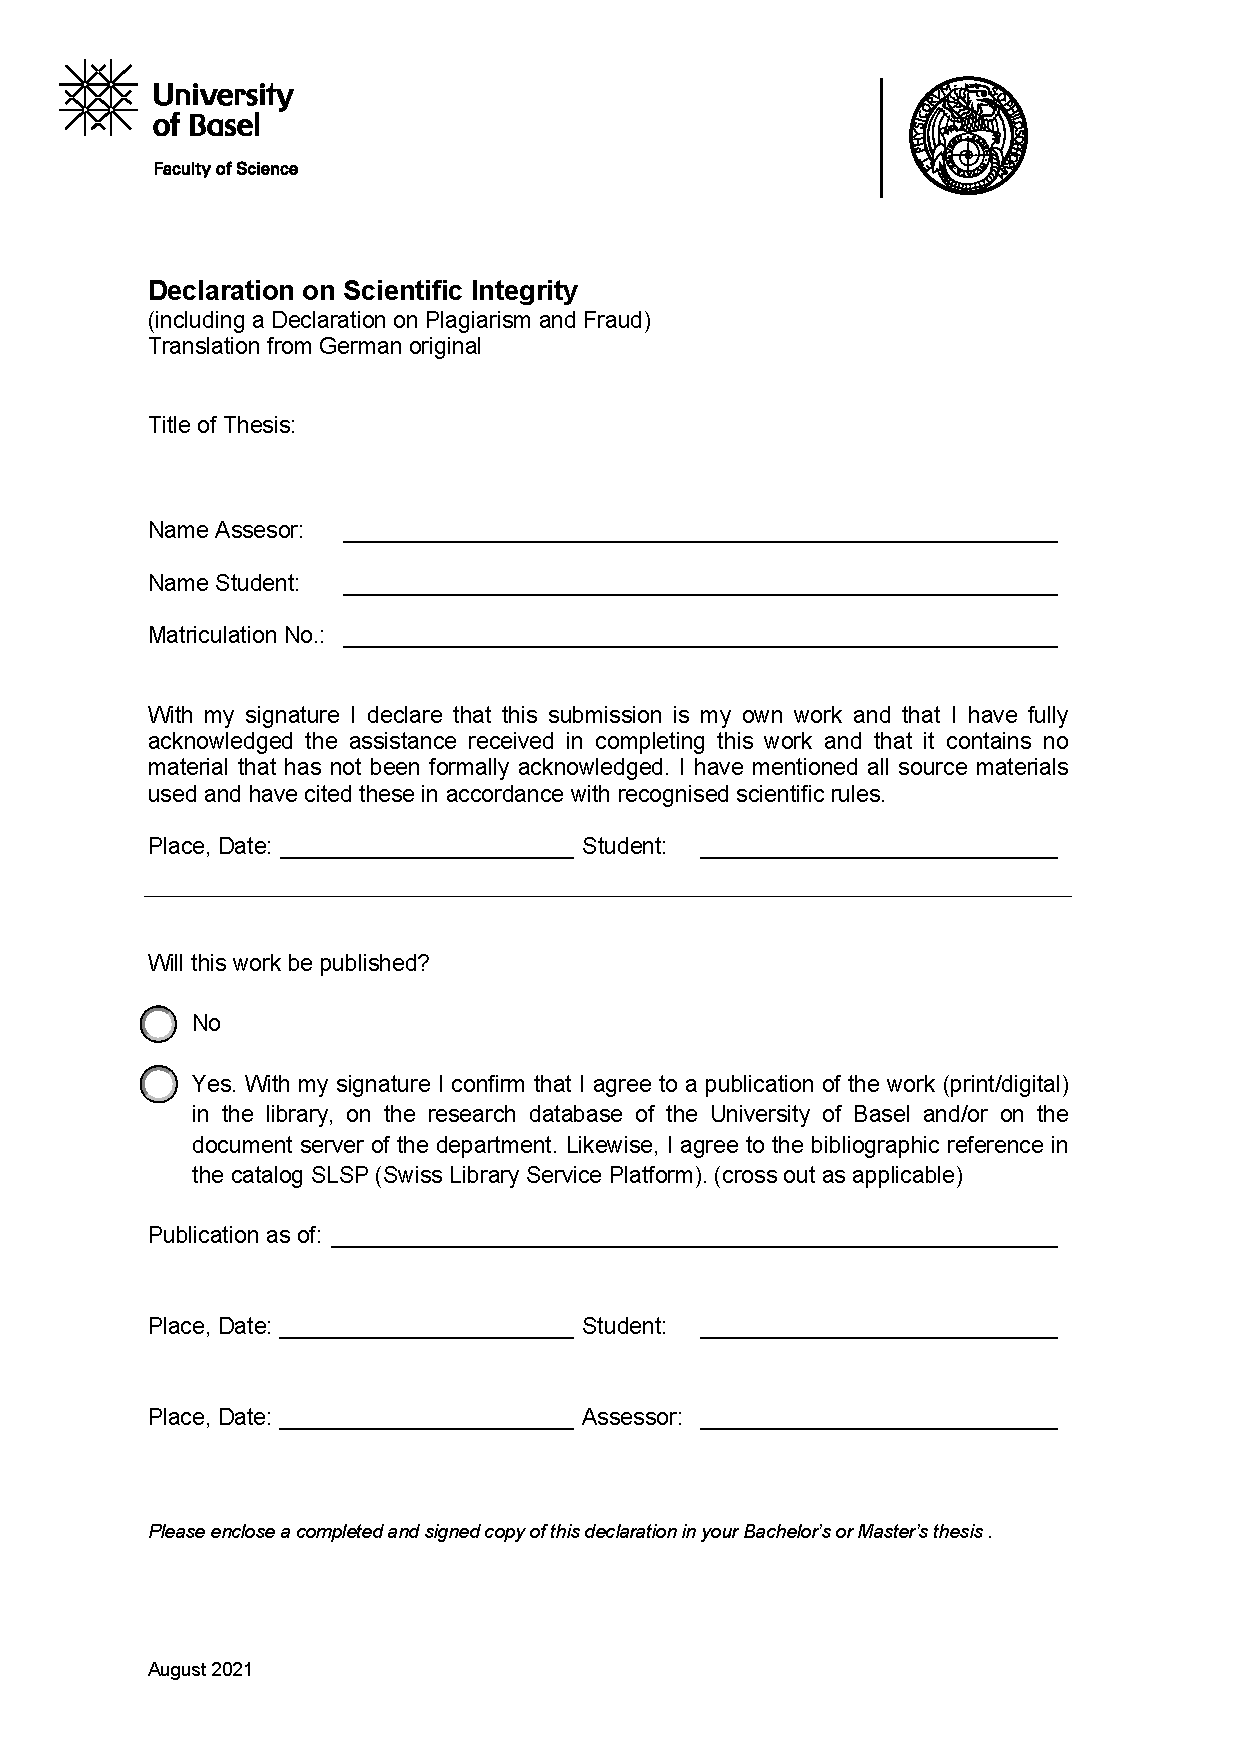
\includepdf{./Back/wissensch_Redlichkeit_E_Aug_21.pdf}}
  {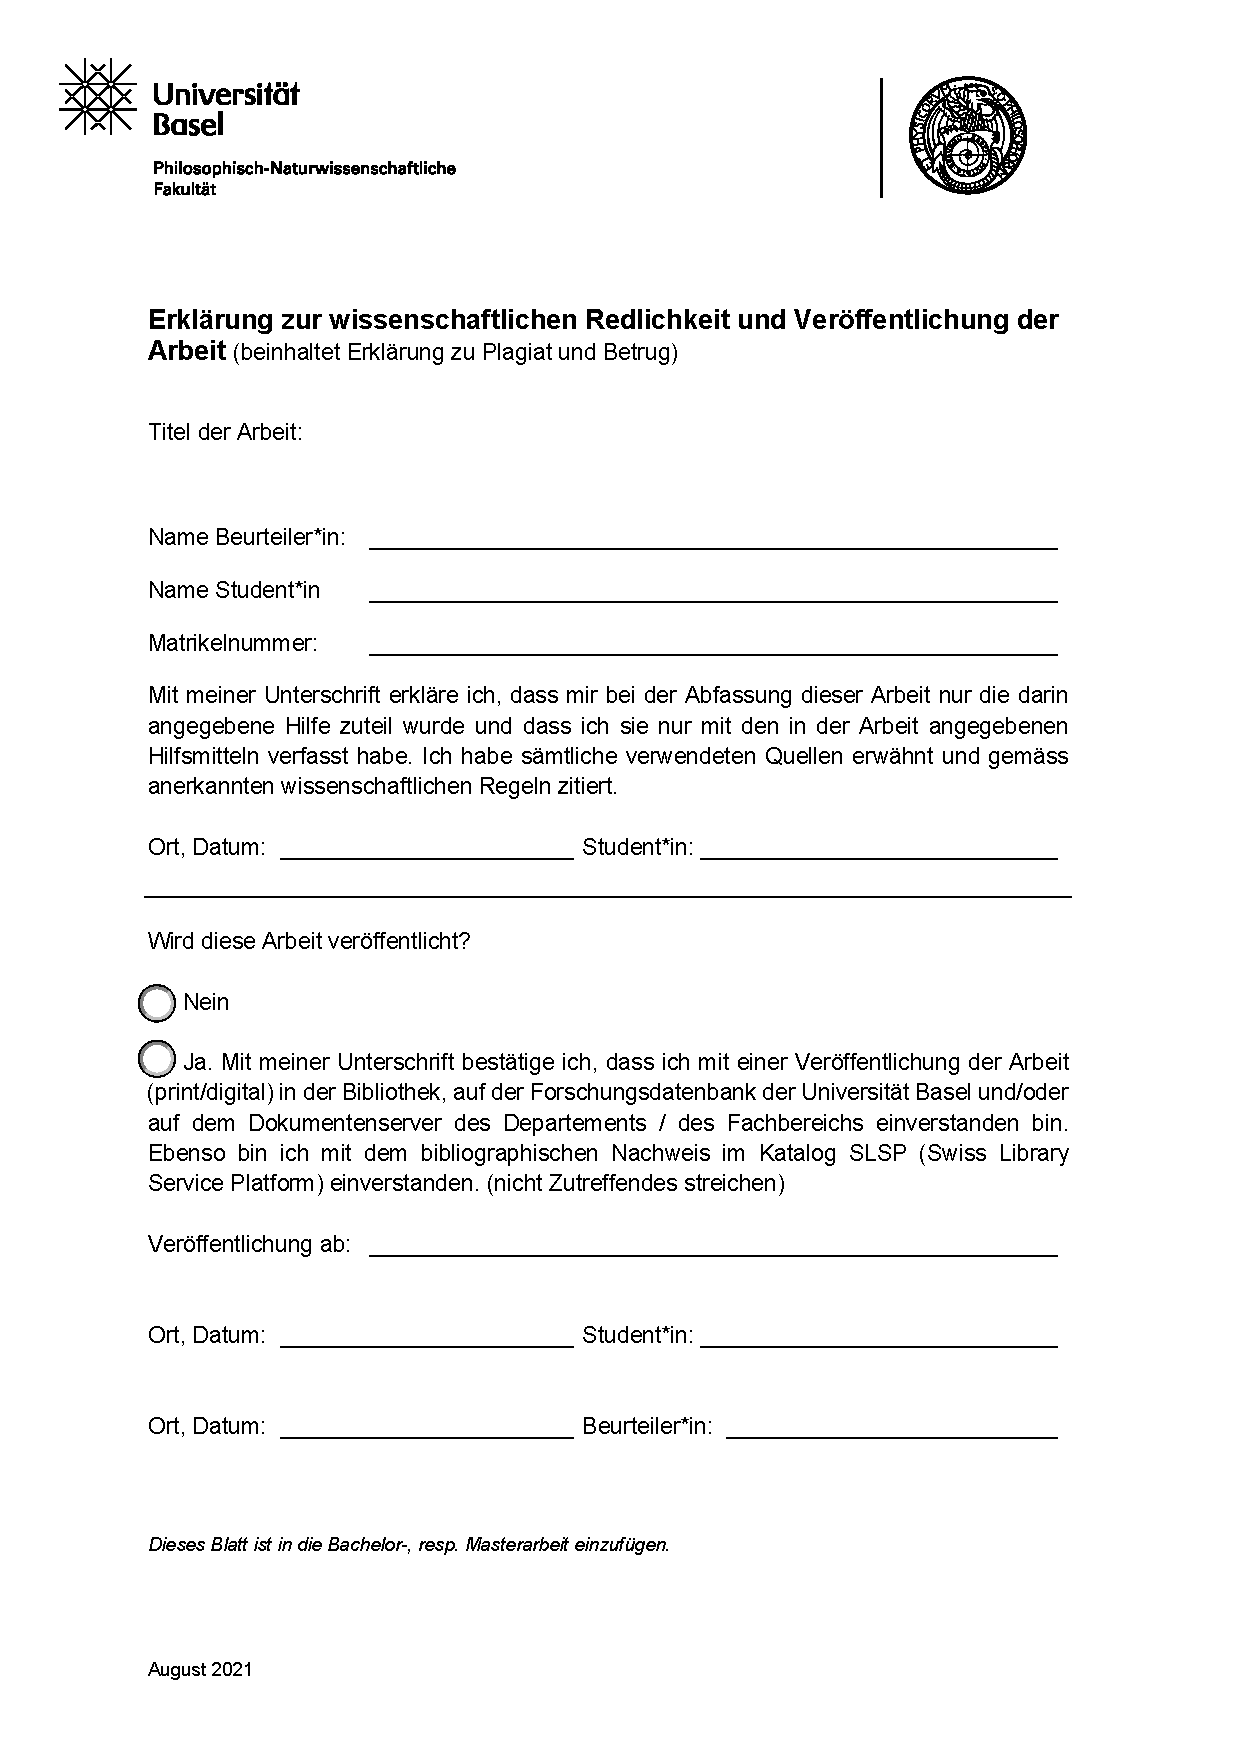
\includepdf{./Back/wissensch_Redlichkeit_D_Aug_21.pdf}}
%% ----------------------------------------------------------------
\end{document}
%% ----------------------------------------------------------------
